\documentclass{report}

% Language packages
\usepackage[utf8]{inputenc}
\usepackage[T1]{fontenc}
\usepackage[portuguese]{babel}

% Code related packages/commands
\usepackage{caption}
\usepackage[newfloat]{minted}

\usepackage{hyperref}


\newcommand{\todo}[1]{{\color{red} #1}}

\title{\todo{A gente descobre depois}}

\author{João Gabriel Trombeta\\
        João Paulo Taylor Ienczak Zanette\\
        Ranieri Schroeder Althoff}
\date{\today}

\begin{document}

\maketitle

\tableofcontents

\chapter{Máquinas Virtuais}

\section{Sobre Máquinas Virtuais}

De maneira sucinta, máquinas virtuais (VM --- \textit{Virtual Machines}) são
computadores sendo executados por outros computadores. Chama-se de
\textbf{Guest} a máquina virtual em si, e de \textbf{Host} o \textit{hardware}
que oferece recursos para executar a VM\@. No host uma cama de software chamada
hypervisor permite a execução de múltiplas máquinas virtuais em uma única
máquina física, independentes e cada uma executando seu próprio SO\@.

\section{Hypervisor}

Também chamado de Monitor de Máquina Virtual (VMM --- \textit{Virtual Machine
Monitor}), um \textbf{Hypervisor} é um componente (seja \textit{hardware},
\textit{software} ou \textit{firmware}) responsável por criar e executar uma
VM, sendo o \textit{Host} o computador em que o Hypervisor é executado.

O Hypervisor é responsável pela camada de abstração entre o host e os guests,
realizando o gerenciamento de recursos, uma vez que cada guest trabalha na
ilusão de que todos os recursos de hardware são seus. Cada VM deve ser isolada
para evitar que uma possa compremeter o funcionamento de outra, por isso toda
interação com o meio físico é intermediada pelo Hypervisor, que é fortemente
protegido das VM\@.

\section{Falhas em Hypervisors}

\subsection{Xen Hypervisor}

Uma falha de segurança detectada com relação a Hypervisors foi explorada no Xen
Hypervisor (criado pelo Xen Project, composto por membros da The Linux
Foundation), em que é possível chamar uma função arbitrária alterando a tabela
de \textit{Hypercalls} (semelhante a uma \textit{vtable}). Uma
\textit{Hypercall} é \textit{software trap} do Hypervisor para executar
operações privilegiadas (como atualizar tabelas de página).

Para explorar a falha, primeiramente é necessário descobrir a localização da
tabela de \textit{Hypercalls}. Para isso, deve-se procurar pela assinatura da
página. Porém, como a página não possui um formato tão previsível, é difícil de
localizá-la (o que é feito pelo \textit{checksum} do conteúdo da página). Em
compensação, a tabela de argumentos dos \textit{Hypercalls} possui um formato
previsível, já que seu conteúdo --- que é o número de argumentos de cada
\textit{Hypercall} --- é fixo, e portanto seu \textit{checksum} também é
previsível. Além disso, a tabela de argumentos sempre se encontra na página
seguinte à tabela de \textit{Hypercalls}, e portanto, ao encontrar uma, se tem
a localização da outra. Aliado à possibilidade de leitura e escrita de código
arbitrário, feito através de falhas nas regras de verificação de segurança de
escrita em páginas do \textit{Hypervision}, é possível então efetuar escape de
máquina virtual (i.e.\ acessar recursos do \textit{Host} que não pertencem à
máquina virtual).

\subsection{VMware ESXi e KVM}

\chapter{AMD Memory Encryption}

\section{AMD Secure Processor}

Grande parte das funções de criptografia executadas em um AMD utilizam um
processador dedicado e independente, o AMD Secure Processor (AMD-SP,
antigamente chamado de Platform Security Processor), que garante que
componentes sensíveis à segurança não recebam interferência do software dos
processadores principais.

O AMD-SP roda um kernel seguro de código fechado, que pode executar tarefas do
sistema assim como tarefas de terceiros confiáveis, tendo o administrador
controle sobre quais tarefas de terceiros são designadas ao processador. Além
disso, o Secure Processor possui uma SRAM dedicada e acesso direto ao CCP, que
é composto por um gerador de números aleatórios, várias engines para o
processamento de algoritmos de criptografia, e um bloco para o armazenamento de
chaves.

\section{Security Memory Encryption}
O AMD Secure Memory Encryption (SME) é um mecanismo que pode ser utilizado para
criptografar os dados que vão para a DRAM, com a finalidade de evitar ataques
físicos. Durante o boot, o AMD Secure Processor gera uma chave que será usada
para criptografar e descriptografar os dados que transitam pela DRAM\@. Como o
a engine de criptografia está dentro do chip o impacto das operações é pequeno.

\begin{figure}[h]
    \centering
    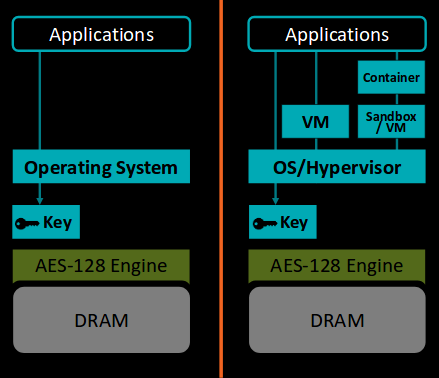
\includegraphics[width=0.5\textwidth]{img/sme}
    \caption{Método de criptografia do SME}\label{sme-1}
\end{figure}

A figura~\ref{sme-1} mostra como ocorre a criptografia. A engine é posicionada
entre o OS/Hypervisor, onde dada a chave o dado é criptografado antes de ser
salvo na DRAM\@. Ao passar da DRAM para o SO novamente, os dados são
descriptografados.

Esse tipo de segurança não previne ataques advindos de um Hypervisor
comprometido, uma vez que ele possui acesso aos dados de maneira direta, esse
tipo de segurança tem com o objetivo evitar ataques como \todo{probe attack na
DRAM}, instalação de hardware que possa acessar a memória do guest, ataques que
possam capturar dados de DIMM e NVDIMM\@.

Para utilizar SME, é necessário verificar se o processador possui suporte para
esse recurso, o que pode ser verificado através da chamada de CPUID
Fn8000\_001F, e que durante o boot o bit 23 de SYSCFG MSR esteja definido como
1 para sinalizar que esse recurso está habilitado. Após isso, ao fazer acesso à
DRAM, é visto o último bit mais significativo do endereço, chamado de C-bit,
que define se o dado deve ou não ser criptografado.

\begin{figure}[h]
    \centering
    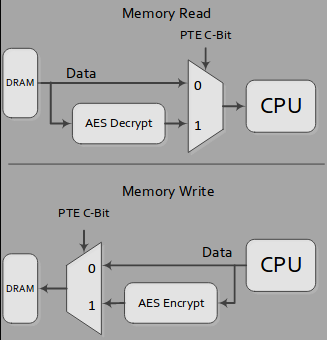
\includegraphics[width=0.5\textwidth]{img/sme_read_write_architecture}
    \caption{Leitura e escrita no SME}\label{sme-read-write}
\end{figure}

Como visto em~\ref{sme-read-write}, para a leitura, antes do dado passar para
CPU, duas versões do dado são inseridas como entrada de um mux, um com o dado
como estava na DRAM e outra com o dado após passar pelo circuito responsável
pela criptografia. O controle do mux recebe o bit mais significativo do
endereço, o C-bit, caso seja 1 significa que o dado está criptografado e a CPU
precisa da informação descriptografada, caso seja 0 significa que o dado pode
ser passado direto para a CPU\@.

Para a escrita a lógica é a mesma, caso o C-bit seja 1 o dado deve ser
criptogrado antes de ser inserido na DRAM, caso seja 0 o dado pode ser salvo
diretamente.

Ainda existe uma variação chamada Transparent SME, onde tudo é criptografado.
Nesse caso não é necessário suporte do SO, tendo em vista que não é preciso
fazer o controle de quais endereços serã criptografados e quais não. O processo
de acesso à memória ocorre da mesma forma que em SME\@.


\section{Secure Encrypted Virtualization}

\section{Aplicação do SME e SEV}

\section{}

\bibliographystyle{ieeetr}
\nocite{*}
\bibliography{references}

\end{document}
